\documentclass[11pt]{article}
\usepackage[T1]{fontenc}
\usepackage{lmodern}
\usepackage{parskip}
\usepackage[colorlinks=true,urlcolor=blue,linkcolor=black,citecolor=black]{hyperref}
\usepackage{graphicx}
\usepackage{amsmath}
\usepackage[utf8]{inputenc}
\usepackage[spanish]{babel}
\usepackage{fancyhdr}
\usepackage{csquotes}
\usepackage{lastpage}
\usepackage{array}
\usepackage{listings}
\usepackage{color}
\definecolor{dkgreen}{rgb}{0,0.6,0}
\definecolor{gray}{rgb}{0.5,0.5,0.5}
\definecolor{mauve}{rgb}{0.58,0,0.82}
\usepackage[affil-it]{authblk}
\usepackage[activate={true,nocompatibility},final,tracking=true,kerning=true,spacing=true,factor=1100,stretch=10,shrink=10]{microtype}
\usepackage[hmargin=2cm,top=4cm,headheight=65pt,footskip=65pt]{geometry}
\usepackage{hyperref}
\usepackage{graphicx}
\usepackage{float}
\usepackage{tabularx}
\graphicspath{ {./screenshots/} }

% Documento
\begin{document}

\begin{titlepage}
 \begin{center}
        \vspace*{1cm}
            
        \Huge
        \textbf{Prácticas de Laboratorio}
            
        \vspace{0.5cm}
        \LARGE
        Informática Forense y Auditoría
            
        \vspace{1.5cm}
            
        \textbf{Hugo Fonseca Díaz}\\
        UO258318\\
        \href{mailto:uo258318@uniovi.es}{uo258318@uniovi.es}
            
        \vfill
            
        Convocatoria Junio-Julio 2021.
            
        \vspace{0.8cm}
            
        
\includegraphics[width=0.3\textwidth]{other/uniovi_logo.jpg}
            
        \Large
        Escuela de Ingeniería Informática\\
        Universidad de Oviedo\\
        España\\
        28 de junio de 2021
            
    \end{center}
\end{titlepage}

\tableofcontents

% Introducción
\section{Introducción}
Los ejercicios de este documento se han realizado en una máquina cuyas características se muestran en la siguiente captura.

\begin{figure}[H]
  \caption{Sistema del alumno Hugo Fonseca Díaz.}
  \centering
    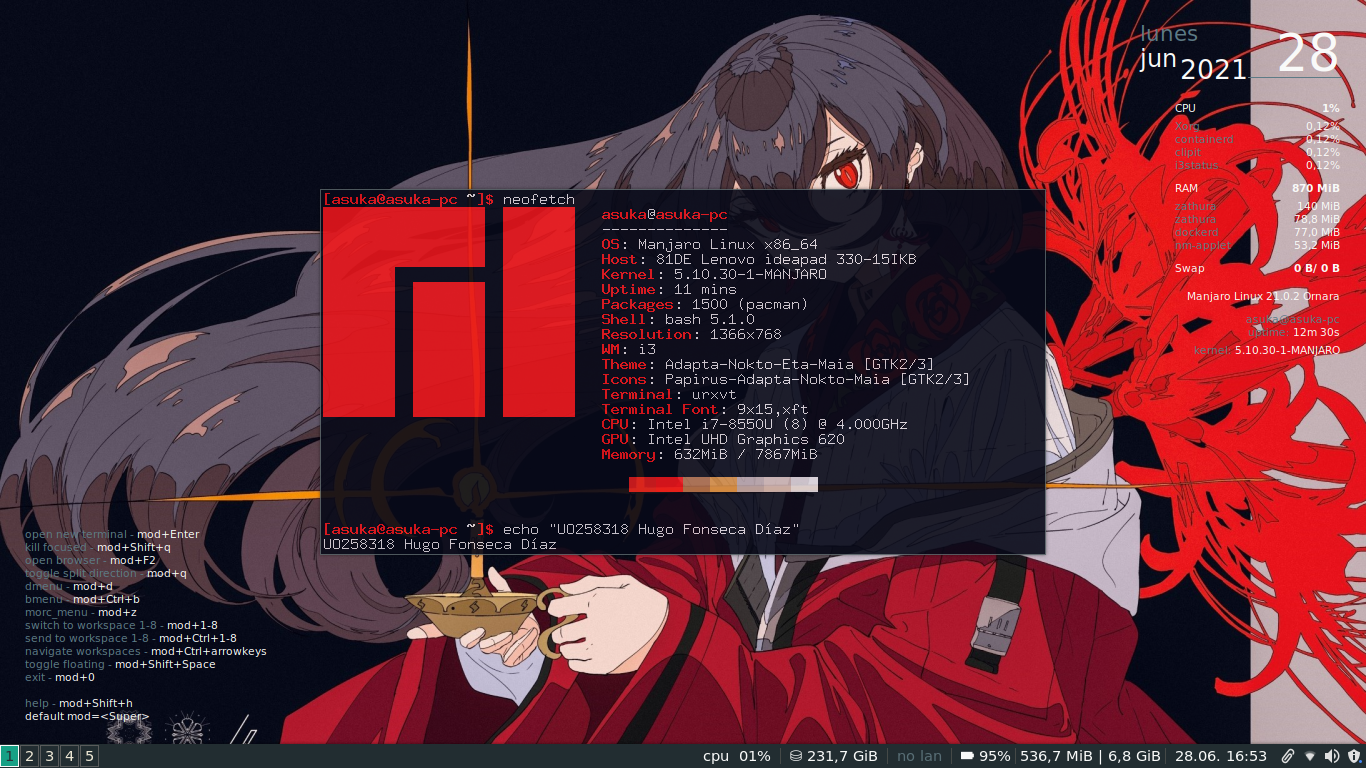
\includegraphics[scale=0.4, trim={0 1cm 0 0}, clip]{other/sistema_hugo.png}
\end{figure}

Las máquinas virtuales utilizadas pueden verse en la siguiente imagen.

\begin{figure}[H]
  \caption{Máquinas virtuales.}
  \centering
    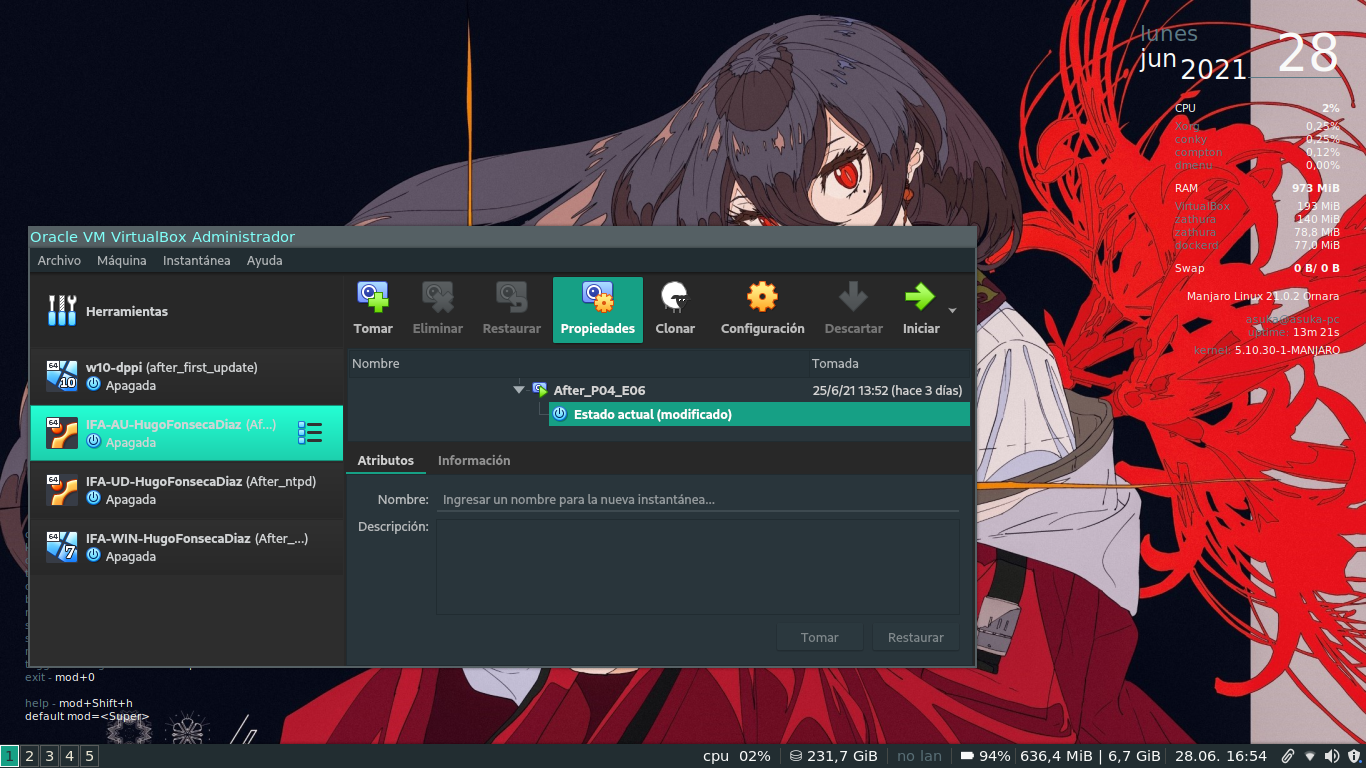
\includegraphics[scale=0.4, trim={0 1cm 0 0}, clip]{other/maquinas_virtuales_hugo.png}
\end{figure}

% Práctica 02
\section{Práctica 02}

% Práctica 03
\section{Práctica 03}

% Práctica 04
\section{Práctica 04}

% Práctica 05
\section{Práctica 05}


\end{document}




